%%%%%%%%%%%%%%%%%%%%%%%%%%%%%%%%%%%%%%%%%%%%%%%%%%%%%%%%%%%%%%%%%%%%
\section{Data Acquisition (DAQ) System Overview}
\label{sec:fd-daq-ov}

\metainfo{DP/SP shared.  Georgia Karagiorgi and Dave Newbold. 2 Pages - largely
  generic but some highlighting of SP-specifics. 
  Focus on describing to HEP but non-DAQ expert. 
  Include how design is resilient in the face of potential
  uncertainties such as excess noise or the need to reduce drift HV
  (just two examples, maybe there are more).}

%%%%%%%%%%%%%%%%%%%%%%%%%%%%%%%%%
\subsection{Introduction}
\label{sec:fd-daq-intro}

The DUNE \dword{fd} \dword{daq} system must enable the readout,
triggering, processing and distribution to permanent storage of data
from all \dwords{detmodule}, which includes both their electrical
\dword{tpc} and optical \dword{pds} signals.  
The final output data must retain, with very high efficiency and low
bias, a record of all activity in the detector that pertains to the
recognized physics goals of the DUNE experiment. 
The practical constraints of managing this output requires that the
\dword{daq} achieve these goals while reducing the input data volume by almost four
orders of magnitude.

The current generation of \dword{lartpc} \dwords{daq}, such as used in
\dword{protodune} and \microboone, produce data spanning a fixed window of
time that is chosen based on the acceptance of an external trigger. 
The DUNE \dword{daq} faces several major challenges beyond those of the
current generation. 
Foremost, it must accept data from about two orders of magnitude more
channels and from that data it must form its own triggers.
This self-triggering functionality requires immediate processing of
the full-stream data from a large portion of all TPC channels with a
throughput of approximately one terabyte per second per
\dword{detmodule}. 
From this data stream, triggers must be raised based on two very
different patterns of activity. 
The first is activity %which is 
localized in a small region of one
\dword{detmodule}, such as due to beam neutrino interactions or the
passage of relatively rare cosmic-ray muons. 
This activity tends to correspond to a relatively large deposition of
energy, around \SI{100}{\MeV} or more. 
The second pattern that must lead to a trigger is lower energy activity
dispersed in both time and spatial extent of the \dword{detmodule}, such as due to a 
\dword{snb}.

The %DUNE \dword{fd} 
\dword{daq} must also contend with a higher order of
complexity compared to the current generation. 
The \dword{fd} is not monolithic but ultimately will consist
of four \dwords{detmodule} each of \nominalmodsize fiducial mass. 
Each module will %follow 
implement somewhat different %unique 
technologies and the
inevitable asymmetries in the details of how data are read out from
each must be absorbed by the unified \dword{daq} at its front end. 
Further, each \dword{detmodule} is not monolithic but has at least one
layer of divisions, here generically named \dwords{detunit}. 
For example, the \dword{sp} \dword{detmodule} has \dwords{apa} each
providing data from a number of \dwords{wib} and the \dword{dp} \dword{detmodule} has
\dword{cro} and \dword{lro} units associated with specific electronics
crates.
In each \dword{detmodule}, there are on the order of \num{100} \dwords{detunit}
(\num{150} for \dword{sp} and \num{245} for \dword{dp}) and each unit has a
channel count that is of the same order as that of an entire \lartpc
detector of the current generation.
The DUNE \dword{daq}, composed of a cohesive collection of \dword{daq} instances
%or really individual instances of the \dword{daq} 
called
\dwords{daqpart}, must run on a subset of all possible
\dwords{detunit} for each given \dword{detmodule}. 
Each instance effectively runs independently of all the others, however
some instances indirectly communicate through the exchange of
high-level trigger information. 
This allows, for example, each \dword{detmodule} to take data in
isolation. It also allows for all \dwords{detmodule} to contribute to forming and
accepting global \dword{snb} triggers, and to simultaneously run small portions -- consisting of a few \dwords{detunit} -- separately in
order to debug problems, run calibrations or %otherwise not disturb
%nominal data taking while maintaining high uptime.
 perform other activities while not interfering with nominal data taking in order to maintain high uptime.

Substantial computing hardware is required to provide the processing
capability needed to identify such activity while keeping up with the
rate of data.
The nature of various technical, financial and physical constraints
leads to the need for much of the computing hardware 
required for this processing
to reside underground, near the \dwords{detmodule}. 
In such an environment, power, cooling, space, and access is far more
costly than in typical data centers. % residing on the surface of the Earth.

Past \lartpc and \dword{lbl} neutrino detectors have successfully
demonstrated external triggering using information related to their beam. %\fixme{FROM their beam operations?}
%associated particle beam. 
%And indeed t
The DUNE \dword{fd} \dword{daq} will accept external information on recent
times of Main Injector beam spills from \fnal. %\fixme{accept spill time information?}
This will assure triggering with high efficiency to capture activity
pertaining to interactions from the produced neutrinos. 

However, even if the DUNE experiment were interested only in 
%had no physics goals other than those related to 
neutrinos from %these 
beam spills, an external beam
trigger alone would not be sufficient. 
Absent any other information, such a trigger must inevitably call for
the readout of all possible data from the \dword{fd} % over a period of time of at least as one \lartpc drift time. 
over at least one \lartpc drift time.
This would lead to an annual data volume approaching an exabyte
($10^{18}$ bytes), the vast majority of which would consist of just noise. 
This entire data volume would have to be saved to permanent storage
and then processed offline in order to get to the signals.

%Of course, DUNE does have a broad set of physics goals which expands to include also theobservation of interactions and decays that are unrelated to the beam of neutrinos from Fermilab. 
DUNE's physics goals of course extend beyond beam-related interactions, including
cosmic-ray muons, which provide an important
source of detector calibration, and atmospheric neutrino interactions,
which give a secondary source from which to measure neutrino
properties. 
Taken together, %and detailed below, 
recording their activity will
dominate the data rate.
The \dword{daq} must also record data with sensitivity to rare interactions
(both known and hypothetical) such as nucleon decay, other baryon
number violating processes (such as neutron-antineutron oscillation),
and interactions from the products of \dwords{snb} as well as possibly
being able to observe isolated low-energy interactions from solar
neutrinos and diffuse supernova neutrinos. 

Some of these events, while rare in themselves, produce patterns of
activity that can be mimicked by other higher-rate backgrounds, particularly
in the case of \dwords{snb}. % this is particularly so. 
While the exact processes involved in \dwords{snb} are not fully understood,
it is expected that a prolonged period of activity of many tens of
seconds will occur over which their neutrino interactions may be
observed. 
Individually, these interactions will be of low energy (relative to
that of beam neutrino interactions, for example), and will be spread
over time and over the bulk of the \dwords{detmodule}. 
Because of their signature and their importance, special attention is
required to first ascertain that a \dword{snb} may be occurring and to save as
much data as possible over its duration.

Thus the \dword{daq} must greatly reduce the full-stream of its input data
while using the data itself to do so. 
It must do this efficiently both in terms of recording essentially all
activity important to the physics goals of DUNE and in terms of a rate of data output 
%data at a rate which 
that is manageable.  
To perform these primary duties the \dword{daq} %requires and will 
provides run
control, configuration management, monitoring of both its processes
and the general health of the data, and a user interface for these activities.
%aspects.  

\subsection{Design Considerations}
\label{sec:fd-daq-des-consid}

The different \dwords{detmodule} vary in terms of their
readout technology and schemes, timing systems, channel counts and data
throughput and format.
%All of this 
These aspects determine the nature of the digital data input
to the \dword{daq}. 
The design of the \dword{daq} strives to contain the unique layers that adapt
to the variation in the \dwords{detmodule} toward its front end in
order to allow as many of its back end components to remain as identical across
the \dwords{detmodule} as possible. 
In particular, the \dword{daq} must present a unified interface to the
ultimate consumer of its data, DUNE offline computing.
It must also accept and process the data from a variety of other
sources including the accelerator, various calibration systems
(including laser, \dword{ce}, \dwords{pd}, and potentially
others) as well as trigger sources external to DUNE.
The modular nature of the DUNE \dword{fd} implies that the \dword{daq} instances running
on each module must also exchange trigger information. 
In particular, exchanging module-local \dword{snb} trigger information
will allow higher efficiency for this important physics.
The \dword{daq} must be optimized for the above while also retaining
the flexibility to scale to handle risks such as excess noise,
changes in \dword{hv}, cut network connectivity and other issues that could arise. %credible potentialities.

\begin{dunefigure}[DAQ overview]{fig:daq-overview}
  {The high-level, \textit{nominal} design for the DUNE \dword{fd} \dword{daq} in
    terms of data (solid) and trigger (dashed) flows between one
    \dword{daqfrag} \dword{fe} and the trigger processing and event
    building back end for one \dword{daqpart}. 
    Line thickness indicates relative bandwidth requirements.
    Blue indicates where the full data flow for the \dword{daqfrag} is
    concentrated to one endpoint.
    Green indicates final output of normally triggered (non-\dword{snb}) data.
    Red indicates special handling of potential \dword{snb}. 
    Each detector module has specialized implementation of some of these
    high level components, particularly toward the upstream \dword{fe}
    as described in the text. 
    The grayed boxes are not in the \dword{daq} scope.
    %See text for details.
  }
% This PDF is made from the .dot of the same name.
% 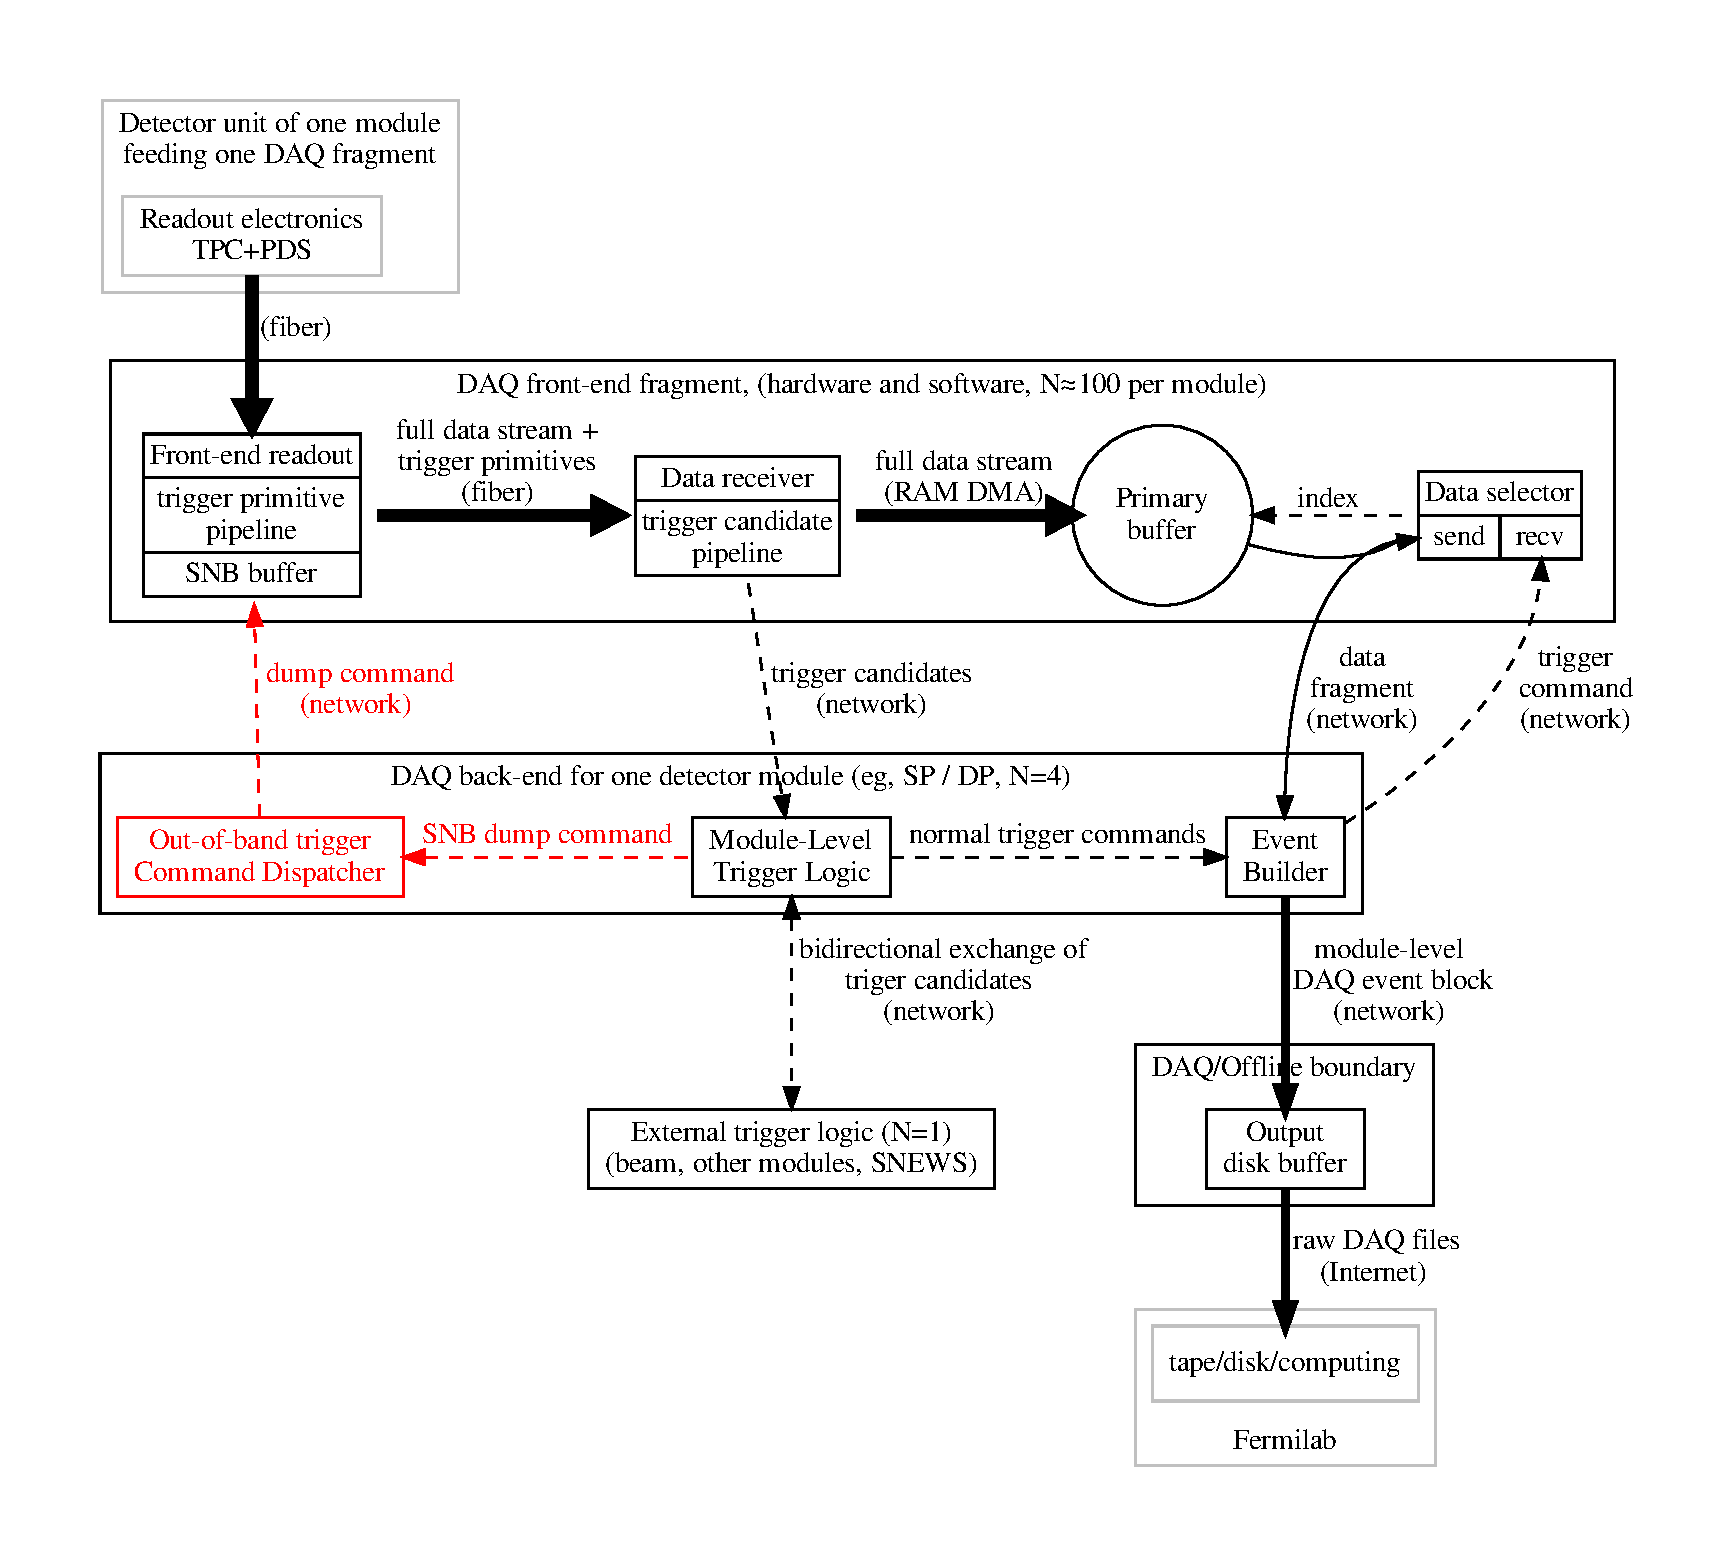
\includegraphics[width=0.8\textwidth]{high-level-daq.pdf}%
  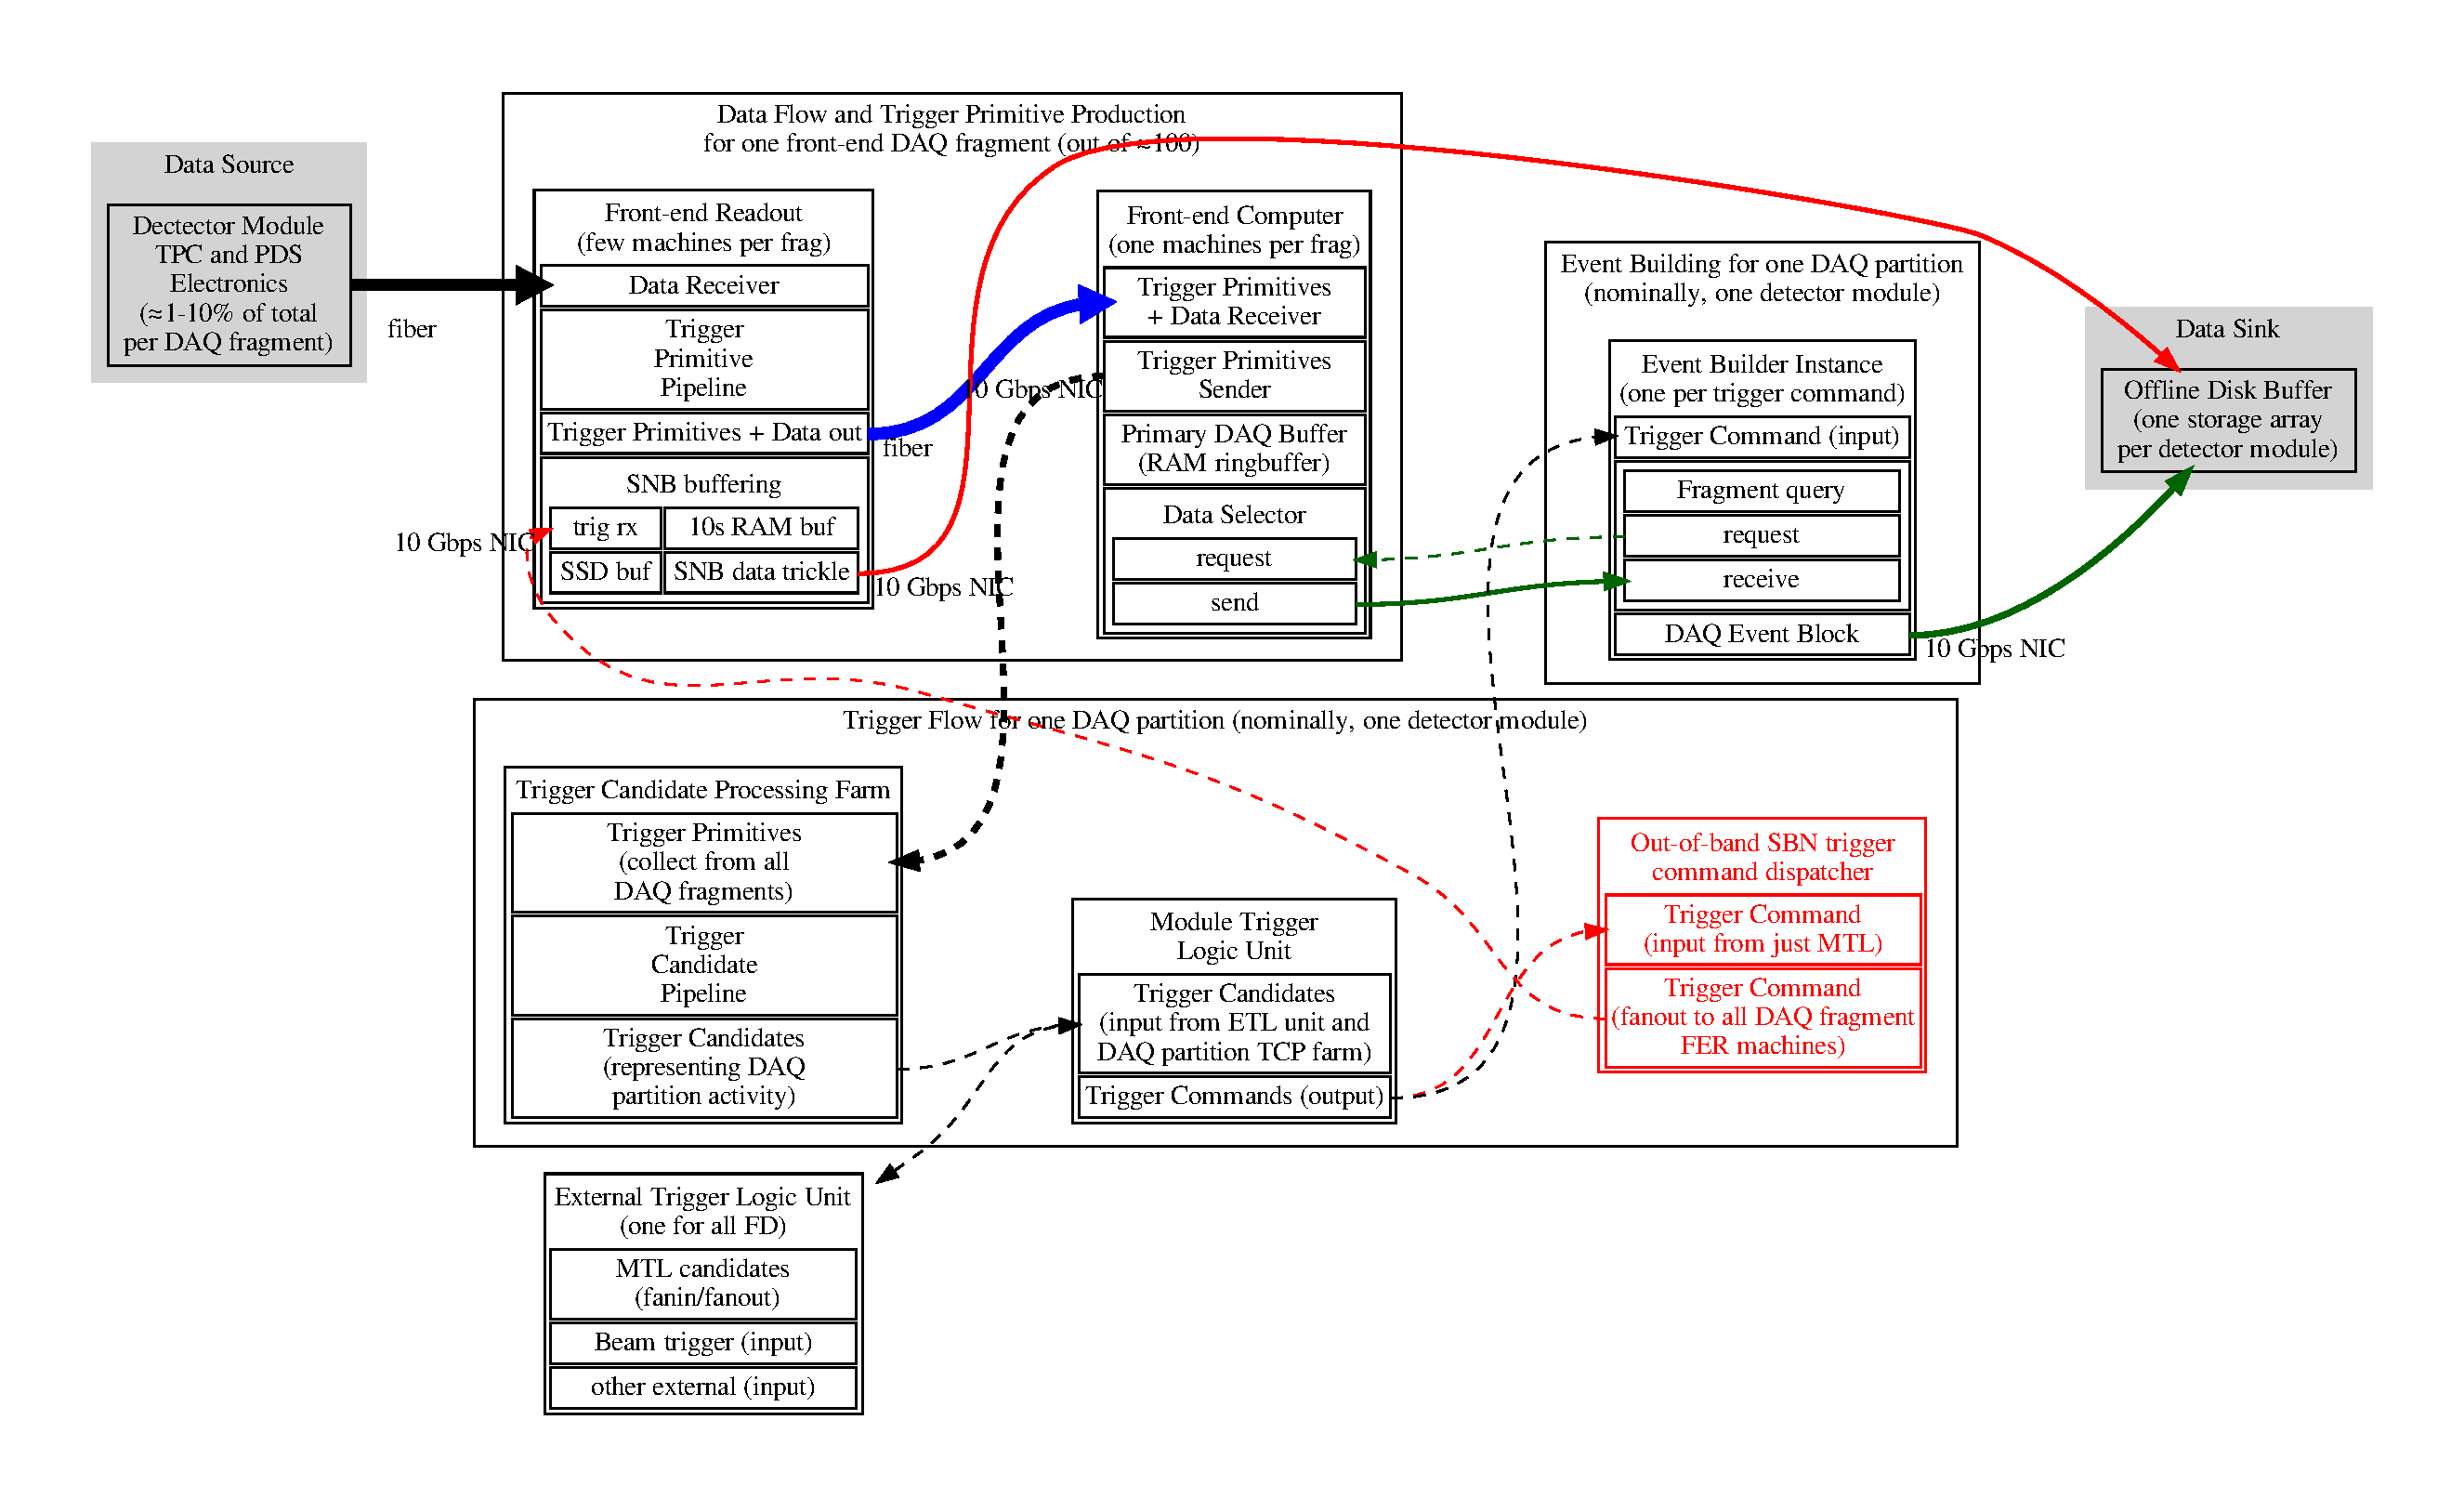
\includegraphics[width=\textwidth{}, trim={1cm 0 1cm 0},clip]{daq-nom-hl.pdf}%
\end{dunefigure}

\begin{dunefigure}[\dword{daq} overview]{fig:daq-overview-alt}
  {The high-level, alternate design for the DUNE \dword{fd}\dword{fd} \dword{daq} in
    terms of data (solid) and trigger (dashed) flows between one
    \dword{daqfrag} \dword{fe} and the trigger processing and event
    building back end for one \dword{daqpart}. 
    Line thickness indicates relative bandwidth requirements.
    Blue indicates where the full data flow for the \dword{daqfrag} is
    concentrated to one endpoint.
    Green indicates final output.
    Note, except for a longer readout, \dword{snb} is handled
    symmetric to normal data.
    Each detector module has specialized implementation of some of
    these high level components, particularly toward the upstream
    front-end as described in the text. 
    The grayed boxes are not in the \dword{daq} scope.
    %See text for details.
  }
% This PDF is made from the .dot of the same name.
% 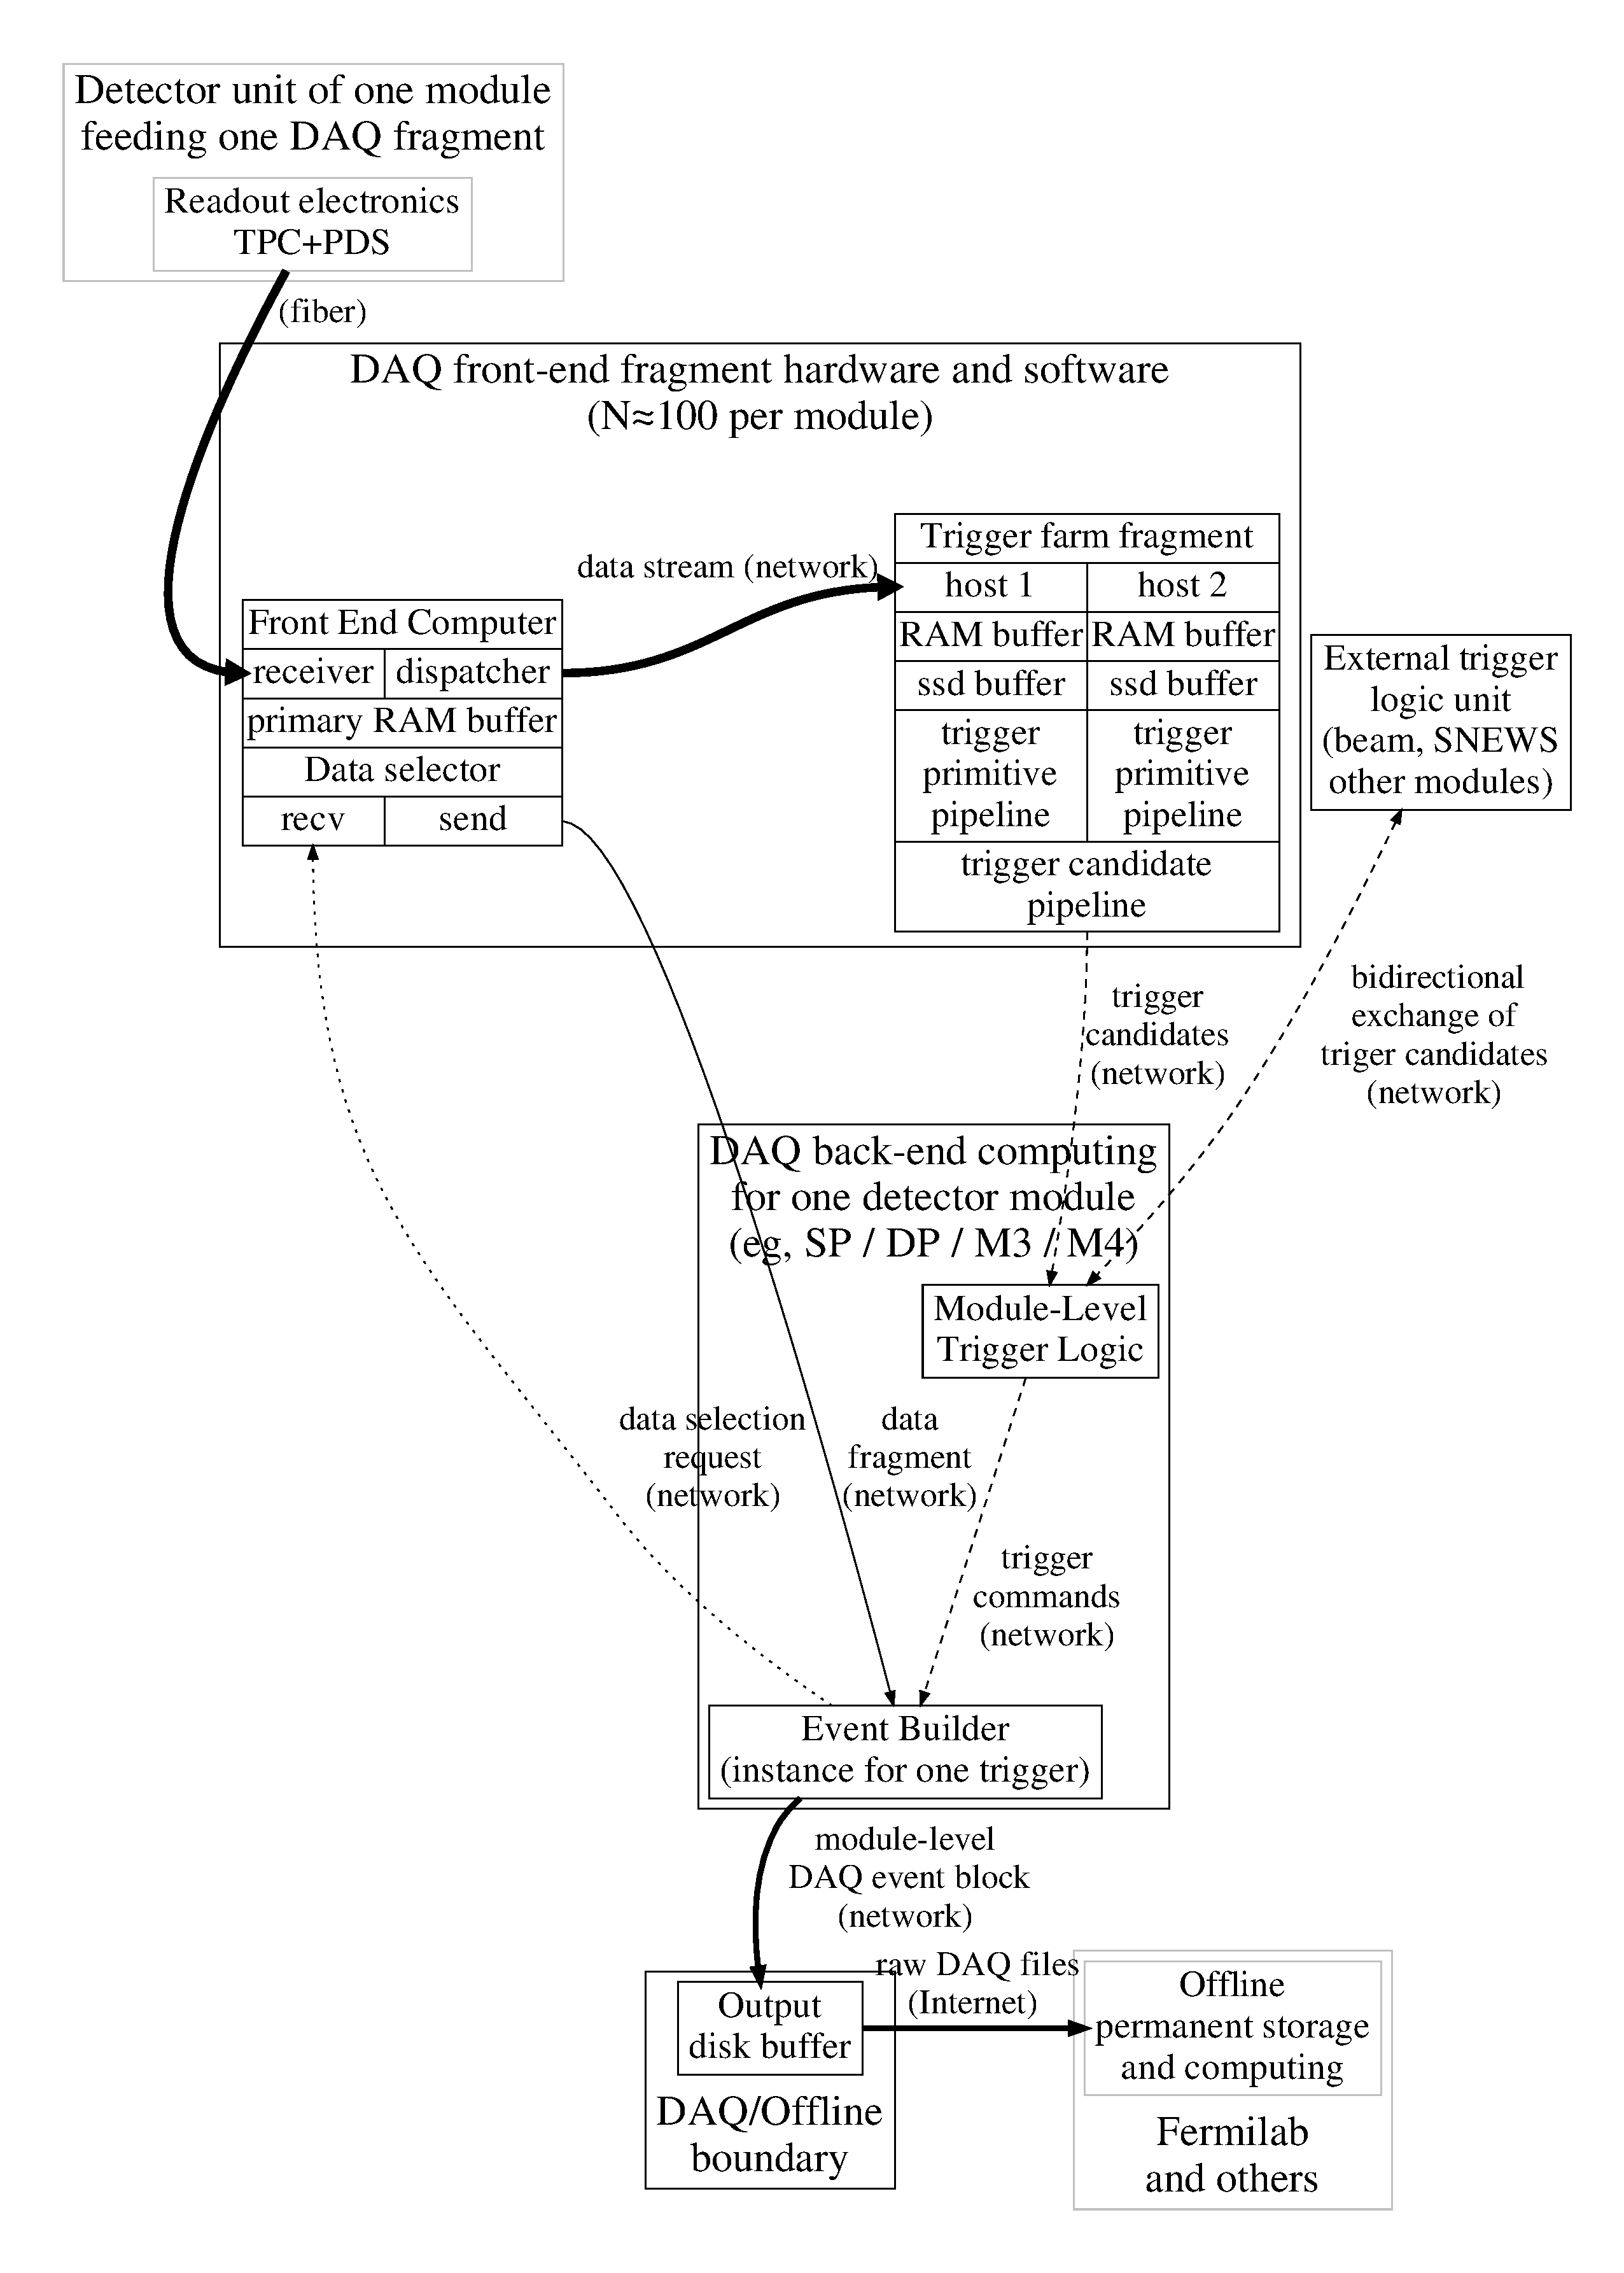
\includegraphics[width=0.8\textwidth]{high-level-daq-alt.pdf}%
  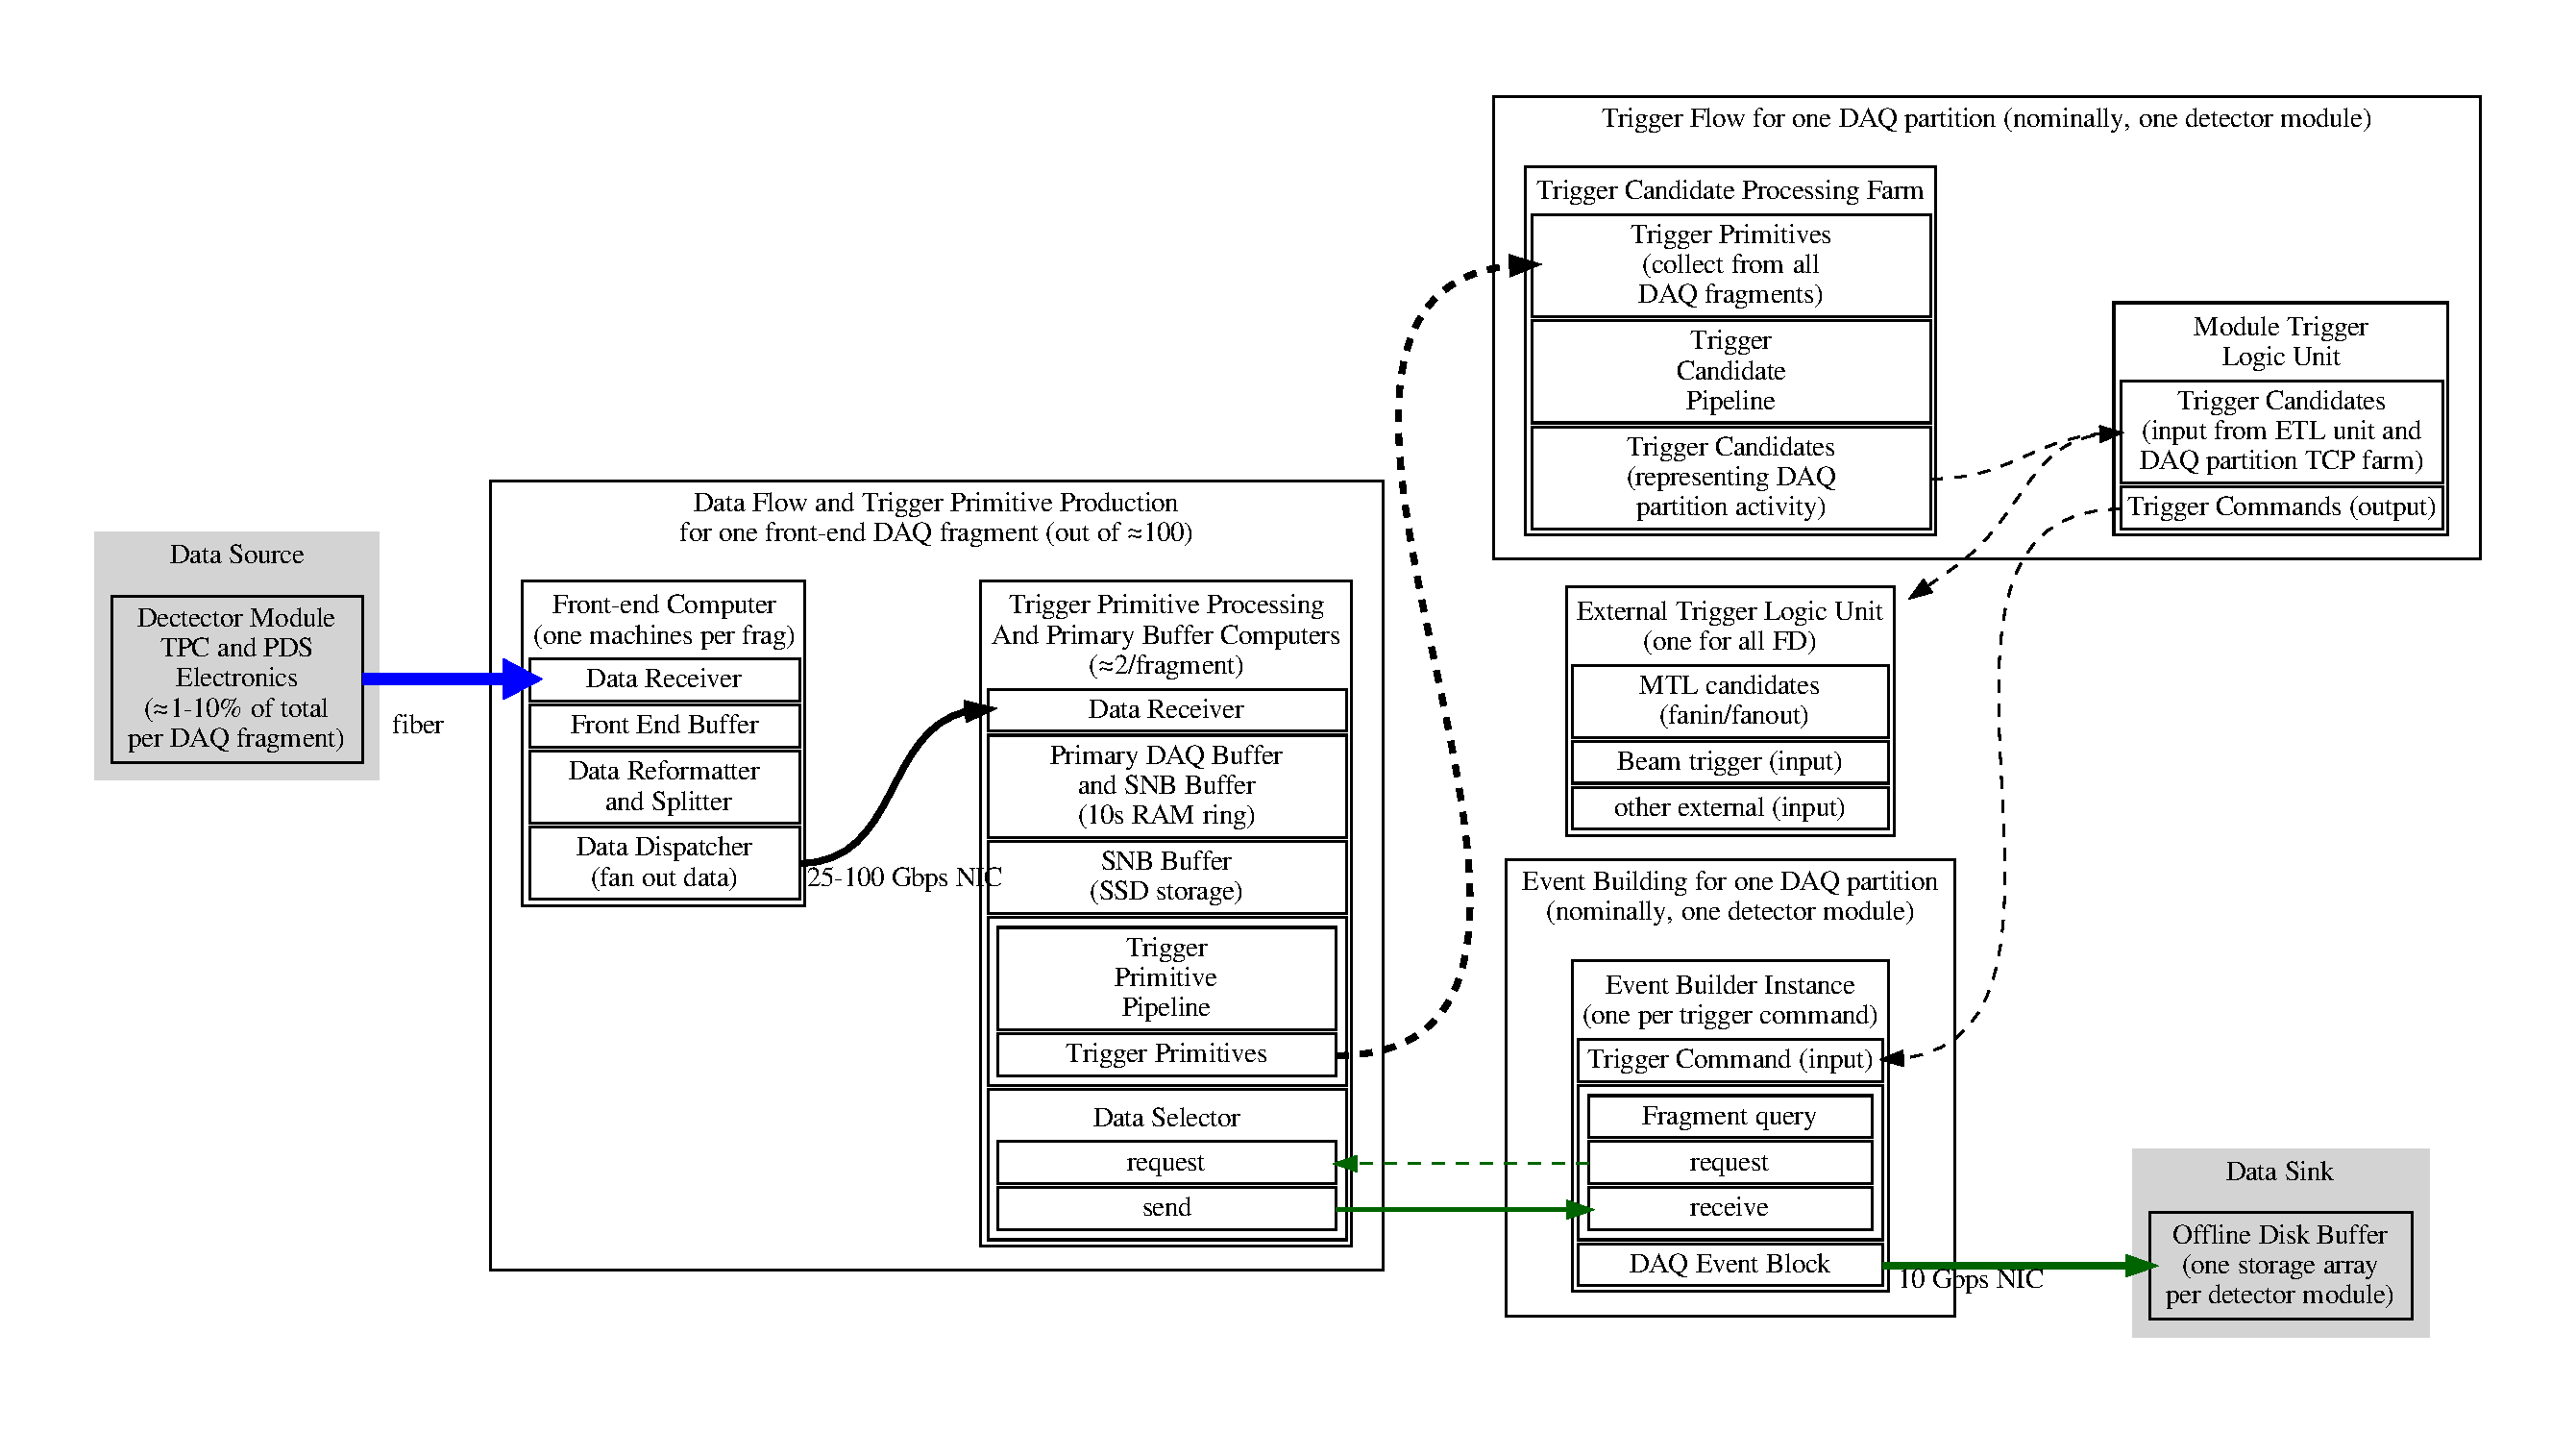
\includegraphics[width=\textwidth{}, trim={1cm 0 1cm 0},clip]{daq-alt-hl.pdf}%
\end{dunefigure}

Currently, two major variations for the DUNE \dword{daq} are under consideration. %being considered. 
The eventual goal is to reduce this to a single high-level design
which will service both \single and \dual \dwords{detmodule} and be reasonably
expected to support the third and forth modules to come.
The first design, designated in this proposal as \textit{nominal}, is
illustrated in a high-level way in terms of its data and trigger flow
in Figure~\ref{fig:daq-overview}. 
The second design, designated as the alternate, is similarly
illustrated in Figure~\ref{fig:daq-overview-alt}. 
The two variants differ largely at their \dwords{fe} in terms of the
order in which they buffer the data received from the \dword{detmodule} 
electronics and use it to form \dwords{trigprimitive}. 
They also differ in how they treat triggering and data flow due to a
potential \dword{snb}. 
As their \dwords{fe} are also sensitive to differences between the
\dword{detmodule} electronics, this further variation for each general
design is described below in Sections~\ref{sec:fd-daq-fero}
and~\ref{sec:fd-daq-fetp} for the \dword{detmodule}  specific to this volume.

At this general high level, the two designs are outlined. % here. 
For both, the diagrams are %drawn 
centered on one \dword{daqfrag}
\dword{fe}, which is a portion of the entire \dword{daqpart} servicing a
\dword{detmodule} that has one \dword{fec} accepting about
\numrange{10}{20}~\si{\Gbps} of data (uncompressed rate) from some integral
number of \dwords{detunit}. 
Each of the participating \dwords{daqfrag} do the following: %provide the actions:
\begin{itemize}
\item Accept TPC and \dword{pds} data from the \dwords{detunit} associated with the \dword{daqfrag}.
\item Produce and emit a stream of per-channel \dwords{trigprimitive}.
\item Buffer the full data stream long enough for the \dword{trigdecision} to complete (at least \snbpretime as driven by \dword{snb} requirements).
\item Accept data selection requests and return corresponding \dwords{datafrag}.
\end{itemize}

All participating \dwords{daqfrag} in the particular \dword{daqpart}
(i.e., the \dword{daq} instance) servicing a portion of one \dword{detmodule}
communicate with one trigger processing and event building system.
The trigger processing system must:
\begin{itemize}
\item Receive the stream of per-channel \dwords{trigprimitive} from all \dwords{daqfrag}.
\item Correlate the primitives in time and spatially (across channels), and otherwise use them to form higher-level \dwords{trigcandidate}.
\item Exchange \dwords{trigcandidate} with the \dword{etl}.
\item From them form \dwords{trigcommand}, each of which describes a
  portion of the data in time and a channel to be read out, such that
  no two trigger commands overlap.
\item Dispatch these commands as required (in general to the \dword{eb}).
\end{itemize}
The event building system is responsible for performing the following actions:
\begin{itemize}
\item Accept a trigger command and allocate one \dword{eb} instance to dispatch it.
\item %The \dword{eb} 
Interpret and execute the command by making
  data selection requests to referenced \dwords{daqfrag}.
\item %The \dword{eb} 
Accept the returned \dword{datafrag} from each
  \dword{daqfrag} and combine them into a \dword{rawevent}.
\item Write the result to the \dword{diskbuffer}, which is the boundary
  shared with DUNE offline computing.
\end{itemize}

The nominal and the alternate \dword{daq} designs differ largely in where
the \dword{trigprimitive} and \dword{snb} buffering exist. 
The \textit{nominal} design places these functions in machines
comprising a \dword{daqfer}, which is upstream of the \dword{fec}. 
This then requires the \dword{snb} data and trigger handling to be
different than that for normal (non-\dword{snb}) data. 
When a \dword{snb} trigger command is raised it is forwarded to the
\dword{daqoob} which sends it down to the \dwords{daqfer}. 
After the \dword{snb} data is dumped to \dwords{ssd} it is
``trickled'' out via a path separate from the normal data to the
\dword{diskbuffer}. 
%
The \textit{alternate} design, on the other hand, places these
functions downstream of the \dword{fec} in trigger processing and data
buffering nodes.
The RAM of these nodes is used to provide the primary \dword{daq} buffer for
normal triggering as well as the deeper buffers needed for \dword{snb}. 
This design handles the \dword{snb} data somewhat
symmetrically with normal data. 
When an \dword{eb} makes a request for \dword{snb} data, it differs
only in its duration, spanning tens of seconds of instead just a few
milliseconds. 
The \dword{fe} buffering nodes, instead of directly attempting to
return the full \dword{sbn} data immediately, streams it to local
\dword{ssd} storage. 
From that storage, the data is sent to the \dword{eb} as low
priority (i.e., also trickled out).
Since the \dword{mtl} ensures no overlapping commands, the buffer
nodes may service subsequent requests from post-dump data that is %will be
in the RAM buffer.
%And, s
Since each trigger command is handled by an individual \dword{eb}
instance, the trickle proceeds asynchronously with respect to any subsequent
trigger command handled by another \dword{eb} instances.

%As mentioned above, f
Further description of %aspects of 
these designs
%, including some of which is specific to a given \dword{detmodule}, 
is
given in Section~\ref{sec:fd-daq-design}.


%The high-level requirements for the DUNE \dword{fd} \dword{daq} are provided in\cite{daq:reqs}.
The most critical requirements for the DUNE \dword{fd} \dword{daq} 
are summarized in Table~\ref{tab:daqrequirements}.

\begin{dunetable}[Important requirements on the \dword{daq} system design]
{p{0.2\textwidth}p{0.6\textwidth}}
{tab:daqrequirements}
{Important requirements on the \dword{daq} system design}   
Requirement  & Description \\ \toprowrule
Scalability & The DUNE \dword{fd} \dword{daq} shall be capable of receiving and
buffering the full raw data from all four \dwords{detmodule} \\ \colhline 
Zero deadtime & The DUNE \dword{fd} \dword{daq} shall operate without deadtime under
\textit{normal} operating conditions \\ \colhline
Triggering & The DUNE \dword{fd} \dword{daq} shall provide full-detector triggering
functionality as well as self-triggering
functionality; the data selection shall maintain high efficiency to
physics events while operating within a total bandwidth of \offsitepbpy
for all operating \dwords{detmodule} \\ \colhline
Synchronization & The DUNE \dword{fd} \dword{daq} shall provide synchronization of
different \dwords{detmodule} to within \SI{1}{$\mu$s}, and of different subsystems
within a module to within \SI{10}{ns}\\ 
\end{dunetable}

The input bandwidth and processing needs of the \dword{daq} are expected to be
dominated by the rate of data produced by the TPC system of each
\dword{detmodule}.
These rates vary between the modules and their estimations are summarized in
Table~\ref{tab:daq-input-bandwidth}.
\begin{dunetable} [Pre-trigger data rates from the  \dword{fd} TPCs and
  into \dword{daq} front end.]
  {lll} {tab:daq-input-bandwidth} {The parameters governing the
    pre-trigger data rate from units of each \dword{detmodule} TPC
    \dwords{ce} and the aggregate throughput into the \dwords{fec} of
    the \dword{daq} \dwords{daqfrag}. 
    Compression is an estimate and will be reduced if excess noise is
    introduced.  
  }
  Parameter & \dlong{sp} & \dlong{dp} \\
  \colhline
  TPC unit & \dword{apa} & \dword{cro} crate \\ \colhline
  Unit multiplicity & \num{150} & \num{240} \\ \colhline
  Channels per unit & \num{2560} (\num{800} collection) & \num{640} (all collection) \\ 
  ADC sampling & \SI{2}{\MHz} & \SI{2.5}{\MHz} \\
  ADC resolution & \num{12}\,bit & \num{12}\,bit \\ \specialrule{1.5pt}{1pt}{1pt}
  Aggregate from \dword{ce} & \SI{1440}{\GB/\s} & \SI{576}{\GB/\s} \\
  Aggregate with compression & \SI{288}{\GB/\s} (5$\times$) & \SI{58}{\GB/\s} (10$\times$)  \\
  \colhline
\end{dunetable}

The ultimate limit on the output data rate of the DUNE \dword{fd} \dword{daq} is
expected to be provided by the available bandwidth to the tape,
disk and processing capacity of \fnal. 
An ample guideline has been established that places this limit at
about \offsitepbpy or \offsitegbps.
Extrapolating to four \dwords{detmodule}, this requires a \dword{daq} data reduction factor of almost four orders of magnitude. 
%this requires the \dword{daq} to perform a data reduction factor of almost four orders of magnitude. 
This is achieved through a simple self-triggered readout strategy.

An overestimate of the annual triggered but uncompressed data volume
for one \nominalmodsize  \dword{detmodule} is summarized in
Table~\ref{tab:daq-data-rates}. 
It assumes a very generous and simple trigger scheme whereby the data
from the entire \dword{detmodule} is saved for a period longer than
two drift times around the trigger time.
This essentially removes any selection bias at the cost of
recording a substantial amount of data that will simply contain noise.
Detailed trigger efficiency studies still remain to be performed. 
Initial understanding indicates that trigger efficiency should be near
\SI{100}{\%} for localized energy depositions of at least \SI{10}{\MeV}. 
Sub-\si{\MeV} signals can be ascertained from noise in existing \lartpc{}s
so the effective trigger threshold may be even lower with high
efficiency. 
Of course, data rates rise quickly when the threshold drops into the
range of an \si{\MeV}. 
Additional simulation and use of early data will be used to better
optimize this threshold.

\begin{dunetable} [Uncompressed data rates for one \dword{spmod}.]
  {p{0.30\textwidth}p{0.13\textwidth}p{0.4\textwidth}}
  {tab:daq-data-rates} {Anticipated annual, uncompressed data rates
    for a single \dword{spmod}. The rates for normal (non-\dword{snb} triggers)
    assume a readout window of \SI{5.4}{\ms}. 
    For planning purposes these rates are assumed to apply to a  
    \dword{dpmod} as well, which has a longer readout time but fewer channels. 
    In reality, application of lossless compression is expected
    to provide as much as a $5\times$ reduction in data volume for the \dword{spmod}
    and as much as $10\times$ for the \dword{dpmod}.}   
  Event Type  & Data Volume \si{\PB/year} & Assumptions \\ \toprowrule
  Beam interactions & \num{0.03} & \num{800} beam and \num{800} dirt muons; \SI{10}{\MeV} threshold in coincidence with beam time; include cosmics\\ \colhline
  Cosmics and atmospherics & \num{10} &  \SI{10}{\MeV} threshold, anti-coincident with beam time \\ \colhline
	 Front-end calibration & \num{0.2} & Four calibration runs per year, \num{100} measurements per point \\ \colhline
 Radioactive source calibration & \num{0.1} & Source rate $\le$\SI{10}{Hz}; single fragment readout; lossless readout \\ \colhline
 Laser calibration & \num{0.2} & \num{1e6} total laser pulses, lossy readout \\ \colhline
 Supernova candidates & \num{0.5} & \num{30} seconds full readout, average once per month \\ \colhline
 Random triggers & \num{0.06} & \num{45} per day\\ \colhline
 Trigger primitives & $\le$\num{6} &  All three wire planes; \num{12} bits per primitive word; \num{4} primitive quantities; $^{39}$Ar-dominated\\ \colhline
\end{dunetable}

The data volume estimates also assume that any excess noise beyond
what is expected due to intrinsic electronics noise will not lead to
an increase in trigger rates. 
If, for example, excess noise occurs such that it frequently mimics
more than about \SI{10}{\MeV} of localized ionization, this would
lead to an increase in various types of triggers and subsequently more
data.
However, at the same time, these estimates do not take into account
that some amount of lossless compression of the TPC data will be
achieved. 
In the absence of excess noise it is expected that a compression
factor of at least $5\times$ can be achieved with the \single data and up
to $10\times$ may be achieved with the \dual data, although the actual  
%Of course, the compression 
factor achieved will ultimately depend on
the level of excess noise experienced in each \dword{detmodule}. 
Studies using data from the DUNE \dword{35t} and early \microboone
running have shown that a compression factor of at least $4\times$ can
be expected even in the case of rather high levels of excess noise.

One category that will be particularly sensitive to excess noise is the trigger primitives. 
As discussed further in Section~\ref{sec:fd-daq-fetp}, their primary
intended use is as transient objects produced and consumed locally
and directly by the \dword{daq} in the \dword{trigdecision} process. 
However, as their production is expected to be dominated by $^{39}$Ar
decays (absent excess noise) they may carry information that proves
very useful for calibration purposes. 
Future studies with simulation and with early data will determine 
 the most feasible methods to exploit this data. 
These may include committing all or a portion to permanent storage or
potentially developing processes that can summarize their data while
still retaining information salient to calibration.

Finally, it is important to note that early data will be used to
evaluate other selection criteria. 
It is expected that efficient and bias-free selections can be
developed and validated that save a subset of the entire
\dword{detmodule} for any given trigger type. 
For example, a cosmic-muon trigger command for a \dword{spmod} will indicate which \dwords{apa}
contributed to its formation (i.e., which ones had local ionization activity). 
This command can then direct reading out these \dwords{apa}, possibly also
including their neighbors, while discarding the data from all other
\dwords{apa}. 
This may reduce the estimated \SI{10}{\PB/year} for cosmics and
atmospherics by an order of magnitude. 
A similar advanced scheme can be applied to the 
\dword{dpmod} by retaining data for the given readout window from
only the subset of \dword{cro} crates (and again, potentially their
nearest neighbors) that contributed to the formation of the given
trigger.



%%%%%%%%%%%%%%%%%%%%%%%%%%%%%%%%
\subsection{Scope}
\label{sec:fd-daq-scope}

%\metainfo{This section may also wish to refer to Fig.~\ref{fig:daq-overview}.}

The nominal scope of the \dword{daq} system is illustrated in
Figure~\ref{fig:daq-overview} by the white boxes. % that are not grayed out. 
It includes the continued procurement of materials for, and the
fabrication, testing, delivery and installation of the following
systems:

\begin{itemize}
\item \dword{fe} readout (nominal design) or trigger farm (alternate
  design) hardware and firmware or software development for
  \dword{trigprimitive} generation.
\item \dword{fe} computing for hosting of \dword{daqdr}, \dword{daqbuf} and \dword{daqds}.
\item Back-end computing for hosting \dword{mtl}, \dword{eb} and the \dword{daqoob} processes.
\item External trigger logic and its host computing.
\item Algorithms to generate trigger commands that perform data selection.
\item Timing distribution system.
\item \dword{daq} data handling software including that for receiving and building 
  events.
\item The \dword{om} of \dword{daq} performance and data content.
\item Run control software, configuration database, and user interface
\item Rack infrastructure in the \dword{cuc} for readout
  electronics, \dword{fe} computing, timing distribution, and data
  selection.
\item Rack infrastructure on surface at \surf for back-end computing.
\end{itemize}
